\documentclass[../main.tex]{subfiles}
% !TeX root = ../main.tex
\begin{document}
	\section{Inventories and Cost of Sales}
	
	For any company to be successful, it must complete its operating cycle 
	efficiently. The operating cycle is a series of activities that a company 
	undertakes to generate revenues and, ultimately, cash. 
	
	\begin{figure}[ht]
		\centering
		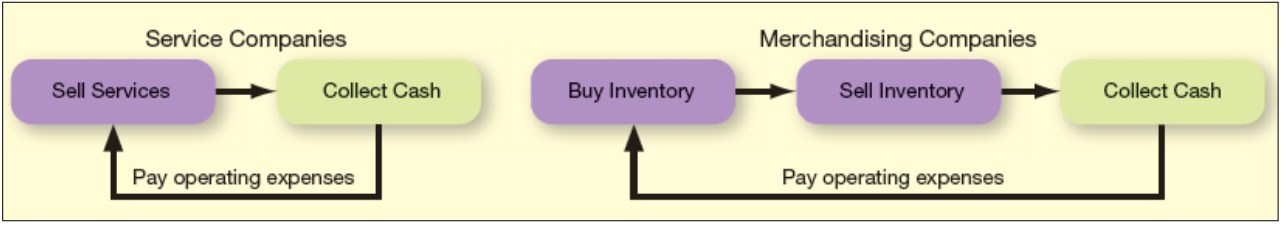
\includegraphics[width=1\columnwidth]{images/c7/operating_cycles.png}
	\end{figure}
	
	\textbf{Service companies} follow a simple operating 
	cycle: sell services to customers, collect cash from them, and use that 
	money to pay for operating expenses.
	
	\textbf{Merchandising companies} differ in that their cycle begins with 
	buying products. These products, which are called \textbf{Inventory}, are 
	sold to customers, which leads to collecting cash that can be used to pay 
	operating expenses and buy more inventory.  
	
	
	There are three key differences in the balance sheet and income statement 
	of a service company \eg Life Time Fitness and a merchandising company 
	\eg Walmart:
	\begin{itemize}[noitemsep]
		\item The balance sheet excerpts. Merchandisers report Inventory as a 
		current asset, but service companies do not. Service companies often 
		report Supplies, but they differ from inventory because supplies are 
		goods acquired for internal use. Inventory consists of goods acquired 
		for resale to customers.
		\item Service companies earn revenue from services whereas 
		merchandisers earn revenue from sales.
		\item Merchandisers report an expense called Cost of Goods Sold, which 
		represents the total cost of all goods sold to customers during the 
		period. Service companies do not incur this expense because they do not 
		sell goods.
	\end{itemize}
	
	\subsection{Inventory Systems}
	Three accounts are particularly important to a merchandiser: 
	\begin{itemize}
		\item \textbf{Inventory} reports the merchandiser’s total cost of 
		acquiring goods that it has not yet sold.
		\item \textbf{Sales Revenue} indicate the total selling price of all 
		goods that the merchandiser did sell to customers during the period.
		\item \textbf{Cost of Goods Sold} cost of all goods that the 
		merchandiser did sell to customers during the period. 
	\end{itemize}

	By subtracting Cost of Goods Sold from Sales Revenue, a merchandiser 
	determines its gross profit, which represents the profit earned before 
	taking into account other expenses such as salaries, wages, depreciation, 
	and so on. 
	\[
	\text{Gross Profit} = \text{Sales Revenue} - \text{Cost of Goods Sold}
	\]
	
	\subsubsection{Balance Sheet and Income Statement Reporting}
	
	Because inventory will be used or converted into cash within one year, it 
	is reported on the balance sheet as a current asset.
	
	\begin{figure}[ht]
		\centering
		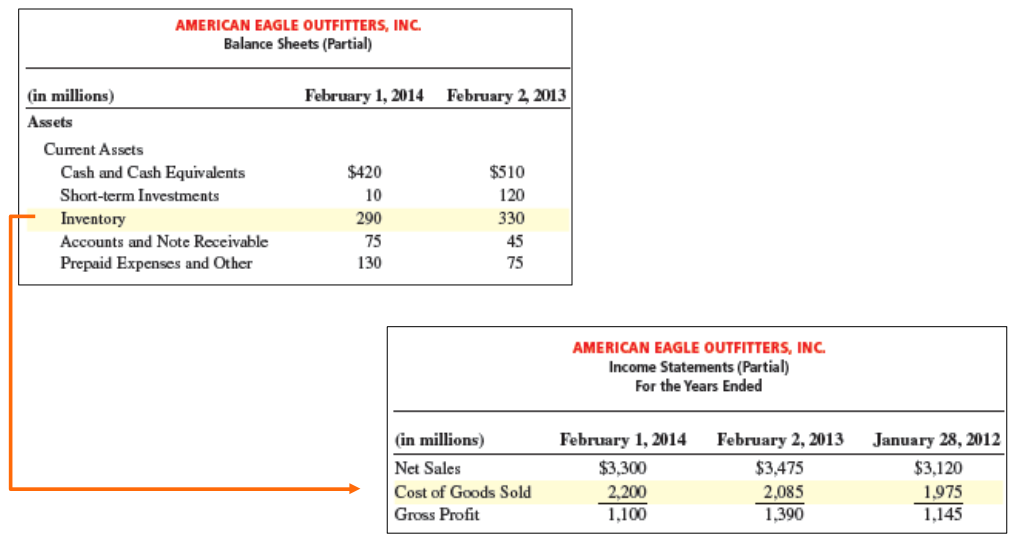
\includegraphics[width=1\columnwidth]{images/c7/inventory_reporting_eg.png}
	\end{figure}
	
	When a company sells goods, it removes their cost from the Inventory 
	account and reports the cost on the income statement as the expense Cost of 
	Goods Sold. Cost of Goods sold is deducted from Net Sales to obtain Gross 
	Profit.
	
	\subsubsection{Inventory Costs}
	
	The \textbf{cost of inventory} includes any cost that is necessary and 
	reasonable to get the inventory to your place of business and to get it in 
	a salable condition.
	
	We already know that the \textbf{invoice price} and \textbf{transportation 
	costs} are included in the total cost of inventory. Other costs to include 
	are \textbf{insurance, storage and import duties}. Any \textbf{purchase 
	discounts} 
	or \textbf{allowances received} reduce the cost of the inventory purchased.
	
	\subsubsection{Perpetual Inventory System}
	
	In a perpetual inventory system, the inventory record are updated 
	perpetually \ie every time an inventory is bought, sold or returned. 
	Perpetual systems are often combined with bar codes and optical scanners. 
	
	\subsubsection{Recording Inventory Purchases}
	
	All inventory-related transactions are recorded in the Inventory account. 
	In general, a purchaser should include in the Inventory account any costs 
	needed to get the inventory into a condition and location ready for sale.
	
	\begin{figure}[ht!]
		\centering
		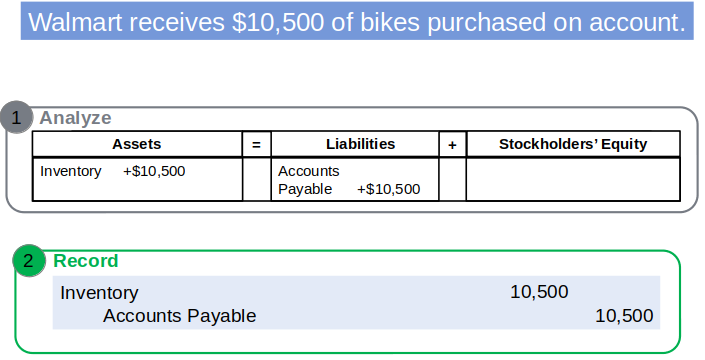
\includegraphics[width=1\columnwidth]{images/c7/inventory_purchases_eg.png}
		\caption{Recording Inventory Purchase}
		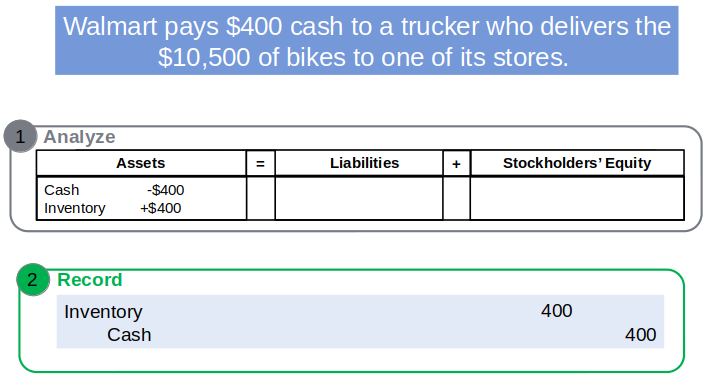
\includegraphics[width=1\columnwidth]{images/c7/transportation_cost_eg.png}
		\caption{Recording Transportation Cost}
		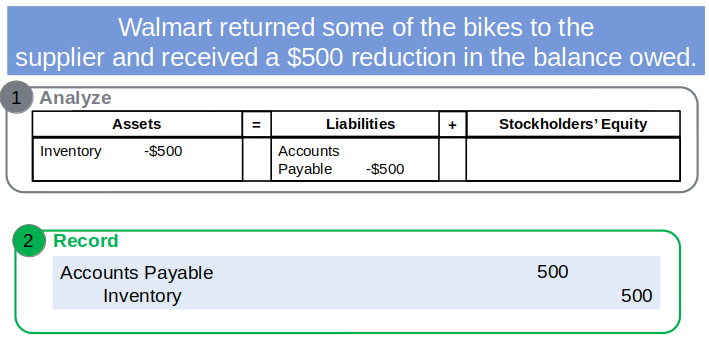
\includegraphics[width=1\columnwidth]{images/c7/purcahse_returns_allowances_eg.png}
		\caption{Purchase Returns and Allowances}
	\end{figure}
	
	When goods purchased from a supplier arrive in damaged condition or fail to 
	meet specifications, the buyer can 
	\begin{itemize}[noitemsep]
		\item Return them for a full refund 
		\item Keep them and ask for a cost reduction, called an 
		\textbf{allowance}.
	\end{itemize}
	Either way, these purchase returns and allowances are accounted for by 
	reducing the cost of the inventory and either recording a cash refund or by 
	reducing the liability owed to the supplier. 
	
	\begin{figure}[ht!]
		\centering
		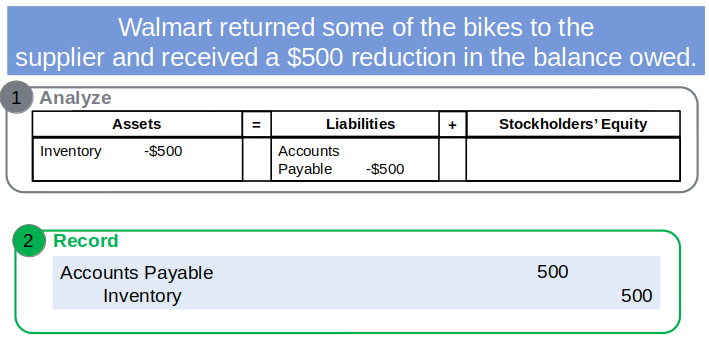
\includegraphics[width=1\columnwidth]{images/c7/purcahse_returns_allowances_eg.png}
		\caption{Purchase Discounts}
	\end{figure}
	
	When inventory is bought on credit, terms such as “2/10, n/30” may be 
	specified. The “2/10” part means that if the purchaser pays by the 10th day 
	of taking ownership of the goods, a 2 percent purchase discount can be 
	deducted from the amount owed. The “n/30” part means that if payment is not 
	made within the 10-day discount period, the full amount will be due 30 days 
	after ownership transferred.
	
		
	\begin{figure}[ht!]
		\centering
		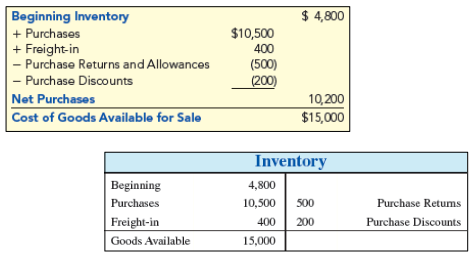
\includegraphics[width=1\columnwidth]{images/c7/inventory_transactions_summary.png}
		\caption{Inventory Transactions Summary}
	\end{figure}
	
	\subsubsection{Recording Inventory Sales}
	
	Merchandisers earn revenues by transferring control of merchandise to 
	customer, either for cash or on credit. 
	
	For a wholesale merchandiser who is shipping goods to a customer, the 
	transfer of control occurs at a time stated in the written sales agreement. 
	The sales agreement will specify one of two possible times:
	\begin{itemize}[noitemsep]
		\item \textbf{FOB shipping point} \ie the sale is recorded when the 
		goods leave the seller’s shipping department.
		\item \textbf{FOB destination} \ie the sale is recorded when the goods 
		reach their destination (the customer).
	\end{itemize}
	
	\begin{figure}[ht!]
		\centering
		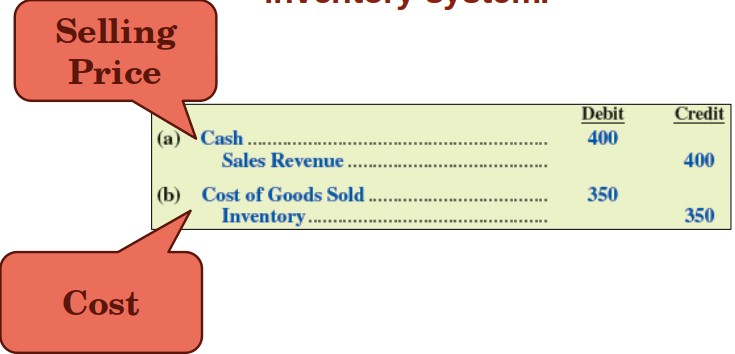
\includegraphics[width=1\columnwidth]{images/c7/recording_sales_eg.png}
		\caption{Recording Merchandise Sale}
	\end{figure}
	
	
	Every merchandise sale has two components, and in a perpetual inventory 
	system, each of these two components require an entry:
	\begin{itemize}
		\item \textbf{Selling price.} An increase in Sales Revenue and a 
		corresponding increase in either Cash (for a cash sale) or Accounts 
		Receivable (for a sale on account).
		\item \textbf{Cost.} The cost that Walmart incurred to initially buy 
		the merchandise is removed from Inventory and reported as an expense 
		called \textbf{Cost of Goods Sold (COGS)}.
	\end{itemize}
	
	\begin{figure}[ht]
		\centering
		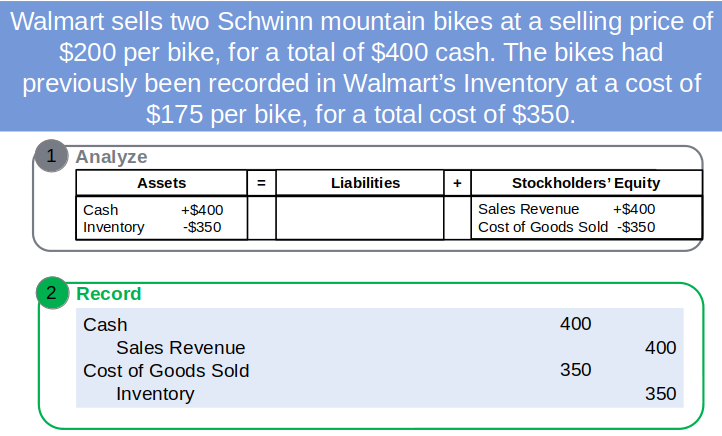
\includegraphics[width=\columnwidth]{images/c7/recording_inventory_sales_eg.png}
	\end{figure}
	
	\subsubsection{Sales Returns and Allowances}
	
	When goods sold to a customer arrive in a damaged condition or are 
	otherwise unsatisfactory, the customer can:
	\begin{itemize}[noitemsep]
		\item Return them for a full refund, or 
		\item Keep them and ask for a reduction in the selling price \ie 
		allowance.
	\end{itemize}
	
	These sales returns and allowances require the merchandising company to 
	revise the previously recorded sale and, in the case of returns, to revise 
	the previously recorded inventory reduction and cost of goods sold.
	
	\begin{figure}[ht!]
		\centering
		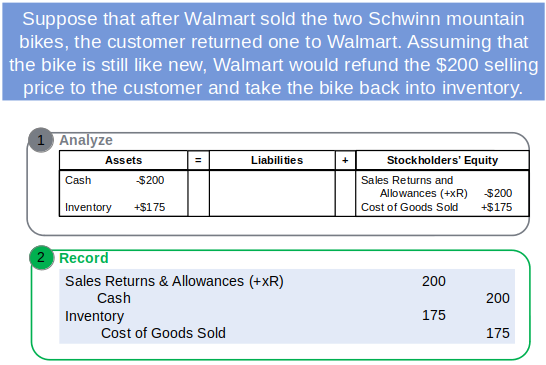
\includegraphics[width=1\columnwidth]{images/c7/sales_return_and_allowance_eg.png}
		\caption{\textbf{Sales Return.} Using a contra-revenue account instead 
		of directly reducing 
		the Sales account allows Walmart to track the value of goods returned, 
		providing clues about whether customers are happy with the quality and 
		price of Walmart ’s products.}	
	\end{figure}

	\begin{figure}[ht!]
		\centering
		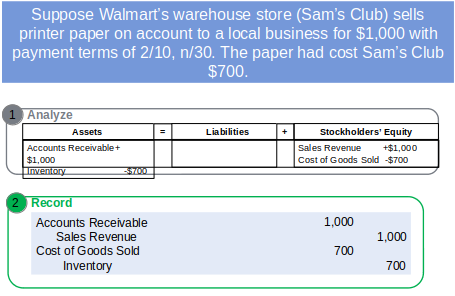
\includegraphics[width=1\columnwidth]{images/c7/sale_discounts_eg.png}
	\end{figure}
	\begin{figure}[ht]
		\centering
		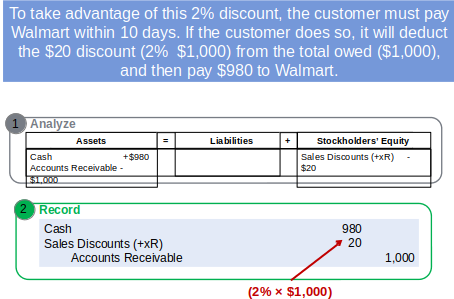
\includegraphics[width=1\columnwidth]{images/c7/sales_discount_eg2.png}
		\caption{Sale Discounts}	
	\end{figure}

	\subsubsection{Summary of Sales Related Transactions}
	
	By using contra-revenue accounts, accountants and managers are able to 
	monitor and control how sales returns, and allowances, and discounts affect 
	the company’s business operations.

	\begin{figure}[ht]
	\centering
	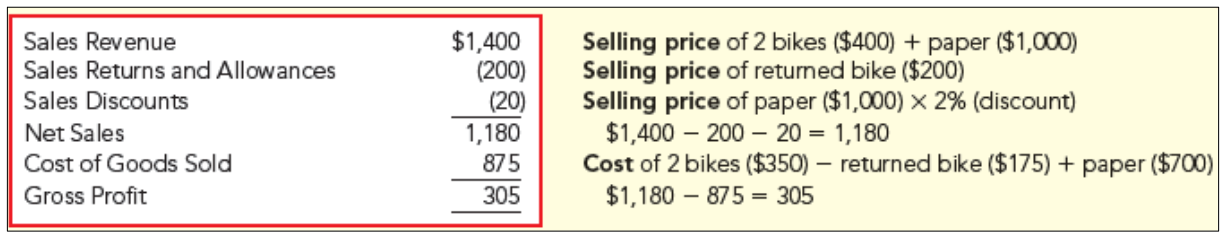
\includegraphics[width=1\columnwidth]{images/c7/summary_sales.png}
	\caption{Sale Summary}	
	\end{figure}

	\subsubsection{Cost of Goods Sold Equation}
	
	A merchandiser starts each accounting period with a stock of inventory that 
	we will call \textbf{beginning inventory (BI)}. During the accounting 
	period, the 
	\textbf{cost of new purchases (P)} is added to the cost of beginning 
	inventory. As 
	in this slide, the sum of these two amounts (BI + P) represents the 
	\textbf{cost of 
	goods available for sale}.
	\[
	\textrm{BI} + \textrm{P} - \textrm{EI} = \textrm{COGS}
 	\]


	Goods available for sale either will be sold 
	during the period (reported as Cost of Goods Sold (COGS) on the income 
	statement) or will remain on hand (reported as \textbf{ending inventory} on 
	the 
	balance sheet). Ending inventory for one accounting period becomes 
	beginning inventory for the next period. 
	
	\[
	\textrm{BI} + \textrm{P} - \textrm{COGS} = \textrm{EI}
	\]

	A cost of goods sold equation can express the relationship among these 
	items in two ways as seen above. If one of the values in the cost of goods 
	sold equation is unknown, you can use either version of the cost of goods 
	sold equation or the inventory T-account to solve for the missing value.
	\begin{figure}[ht]
		\centering
		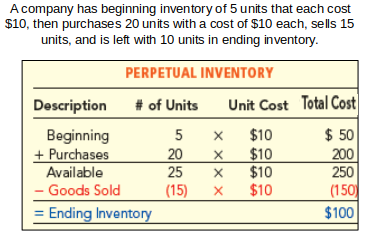
\includegraphics[width=1\columnwidth]{images/c7/cogs_equation.png}
		\caption{\textbf{COGS Equation Example.} In a perpetual inventory 
		system, the Cost of Goods Sold is updated with each inventory 
		transaction, which “forces” out” the cost of ending Inventory.}	
	\end{figure}
	
	\subsection{Inventory Cost Flow}
	
	Management decisions in accounting for inventory involve the following:
	\begin{itemize}[noitemsep]
		\item Items included in inventory and their costs.
		\item Costing method \eg specific identification, FIFO, or weighted 
		average cost\footnote{LIFO is not allowed under IFRS}
		\item Inventory System (perpetual or periodic)
		\item Use of market values or other estimates
	\end{itemize}
	
	Choices made concerning these four points affect the reported amounts for 
	inventory, cost of goods sold, gross profit, net profit, current assets, 
	and other accounts.  
	
	Under IFRS, three methods are commonly used to assign costs to inventory 
	and to cost of goods sold. Each method has a \textbf{cost flow assumption}:
	\begin{itemize}[noitemsep]
		\item \textbf{Specific Identification} - can be used when each item can 
		be identified with a specific purchase
		\item \textbf{Last-in, First-out (LIFO)} 
		\item \textbf{First-in, First-out (FIFO)} - assumes costs flow in the 
		order incurred
		\item \textbf{Weighted Average Cost} - assumes costs flow at the 
		average of the costs available.
	\end{itemize}
	Each method assumes a particular pattern for how costs flow through 
	inventory. Each of these three methods is acceptable whether or not the 
	actual physical flow of goods follows the cost flow assumption. 
	
	\begin{figure}[ht]
		\centering
		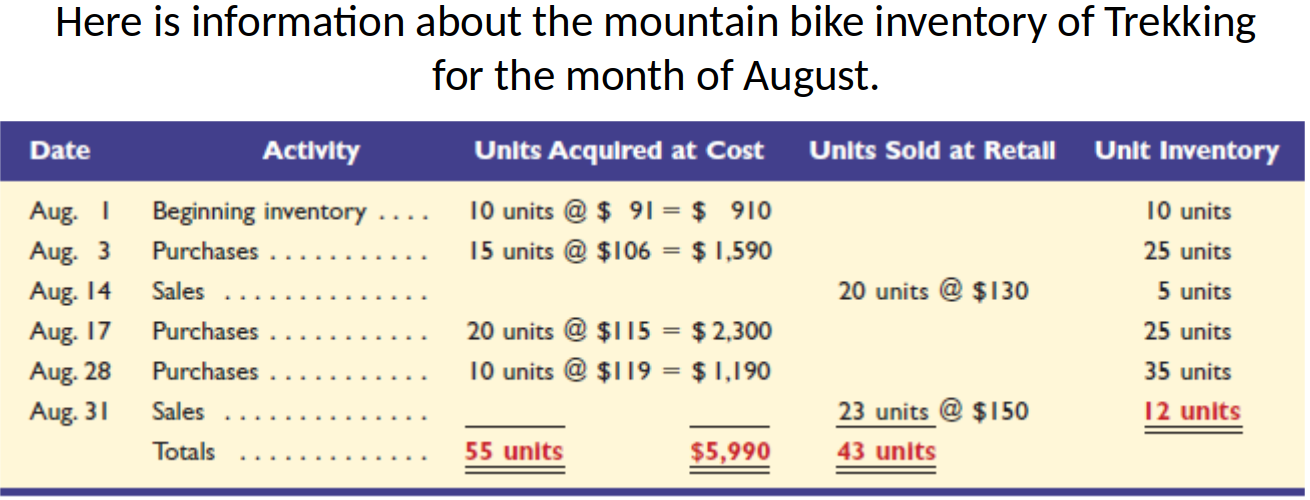
\includegraphics[width=\columnwidth]{images/c7/inventory_costing_eg.png}
	\end{figure}
	
	\subsubsection{Specific Identification}
	
	In this method, we know the specific cost of each unit that is sold. It is 
	most commonly used in businesses that have low sales volume of high dollar 
	items, like car dealerships, exclusive jewelry stores, and custom builders.
	
	\begin{figure}[ht]
		\centering
		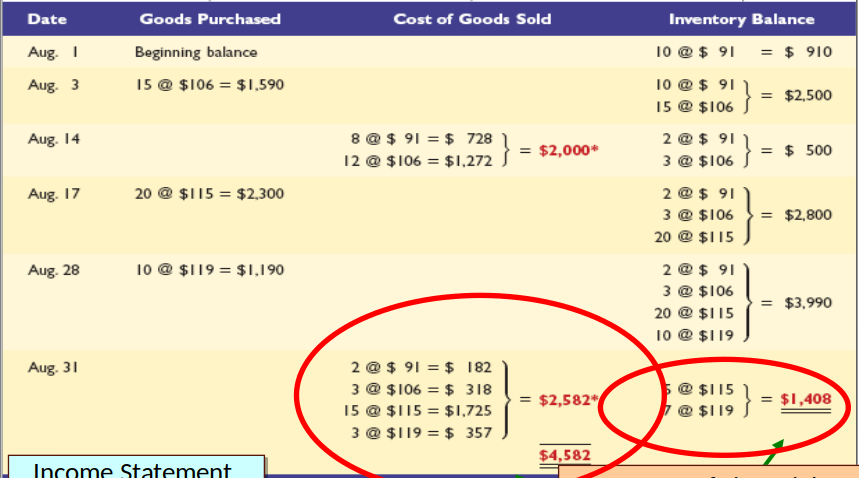
\includegraphics[width=\columnwidth]{images/c7/specific_id.png}
		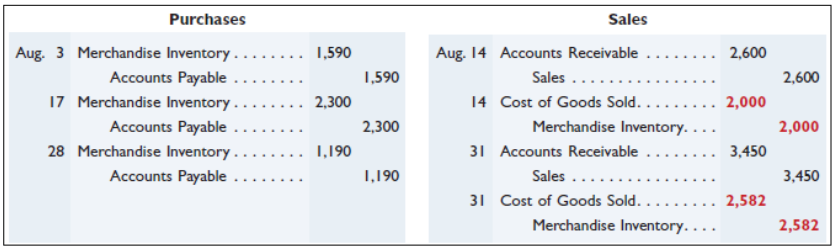
\includegraphics[width=\columnwidth]{images/c7/specific_id_eg1.png}
		\caption{Specific Identification}
	\end{figure}

	\subsubsection{First-In, First-Out (FIFO)}
	
	When using FIFO, we assign the older costs to the units sold. That leaves 
	the more recent costs to be used to value ending inventory.
	
	\begin{figure}[ht]
		\centering
		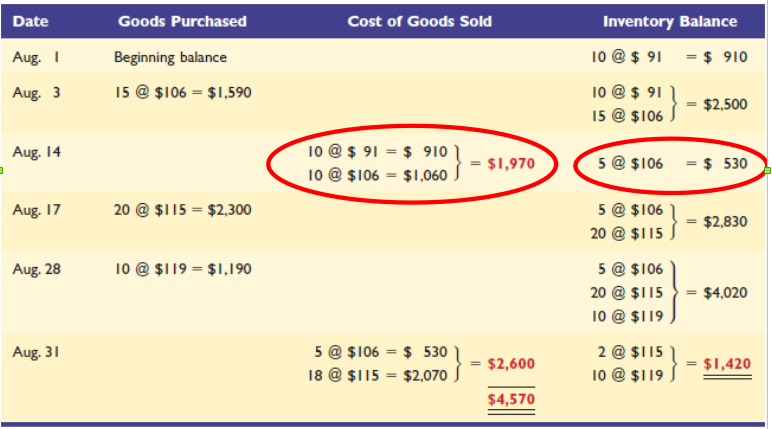
\includegraphics[width=\columnwidth]{images/c7/fifo.png}
		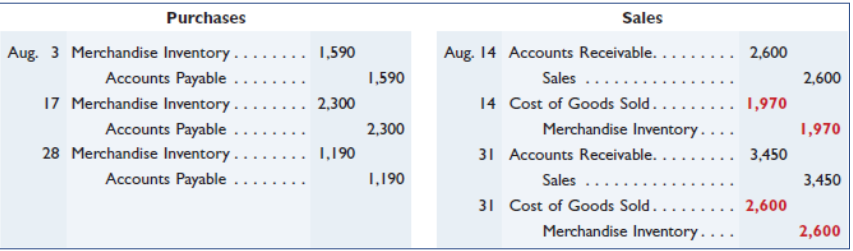
\includegraphics[width=\columnwidth]{images/c7/fifo_eg1.png}
		\caption{FIFO}
	\end{figure}
	
	\subsubsection{Weighted Average Cost}
	
	When using weighted average cost, we assign the average cost of the goods 
	available for sale to cost of goods sold.  The average cost is determined 
	by dividing the cost of goods available for sale by the units on hand.  
	
	\begin{figure}[ht]
		\centering
		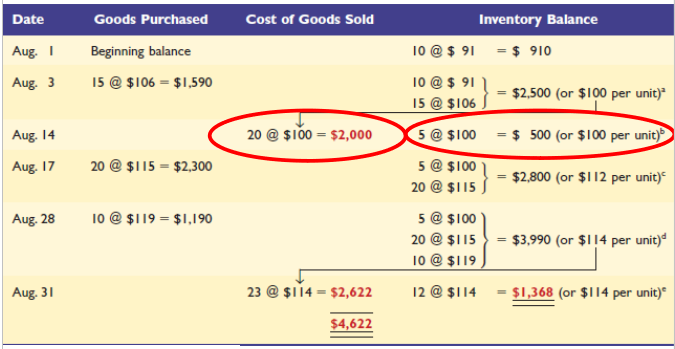
\includegraphics[width=\columnwidth]{images/c7/weighted_average_cost.png}
		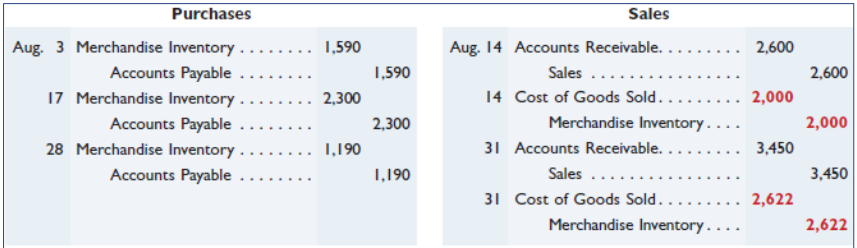
\includegraphics[width=\columnwidth]{images/c7/weighted_average_eg1.png}
		\caption{Weighted Average Cost}
	\end{figure}
	
	First, we need to compute the weighted average cost of the items in 
	inventory. We do this by dividing the cost of goods available for sale of 
	by the total units in inventory.
	
	\subsubsection{Financial Statement Effects of Costing Methods}
	
	Because prices change, inventory methods nearly always assign different 
	cost amounts. 
	
	\begin{figure}[ht]
		\centering
		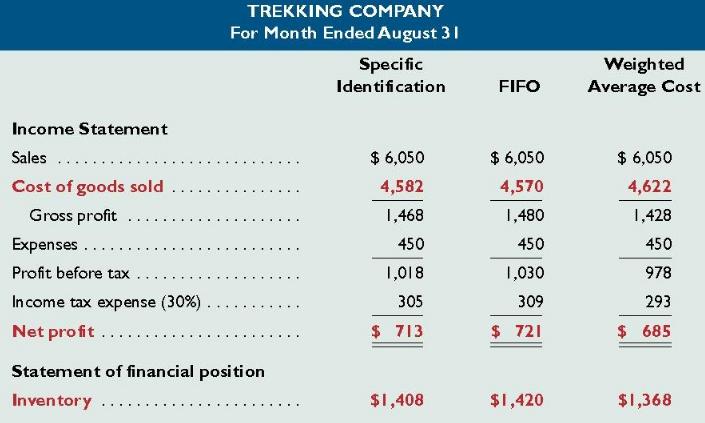
\includegraphics[width=\columnwidth]{images/c7/costing_comparison.png}
		\caption{Costing Method Comparisons}
	\end{figure}
	
	In periods of rising prices, of the other two methods, FIFO will provide 
	the lower Cost of Goods Sold amount. This is because it uses the older 
	costs which tend to be lower to arrive at this amount. Weighted average 
	will provide a Cost of Goods Sold amount that is higher. As you can see, 
	the impact on net profit is that FIFO results in the higher net profit, and 
	weighted average cost results in lower net profit.  
	
	\subsubsection{Lower of Cost and Net Realizable Value}
	
	\textbf{Net Realizable Value (NRV)} is the estimated selling price in the 
	ordinary course of business less the estimated costs of completion and the 
	estimated costs necessary to make the sale. NRV can be applied in two ways:
	\begin{itemize}[noitemsep]
		\item Separately to each individual item.
		\item To major categories of assets. 
	\end{itemize}
	
	When we report inventory on the statement of financial position, we report 
	it at the lower of cost and NRV. Cost is determined using one of the 
	methods we just discussed: Specific identification, FIFO, or weighted 
	average cost. The \textbf{market} is defined as the current replacement 
	price of the inventory. This way of valuing inventory is also known as the 
	\textbf{Lower of Cost and Market Value (LCM) Rule}.
	
	\begin{figure}[ht]
		\centering
		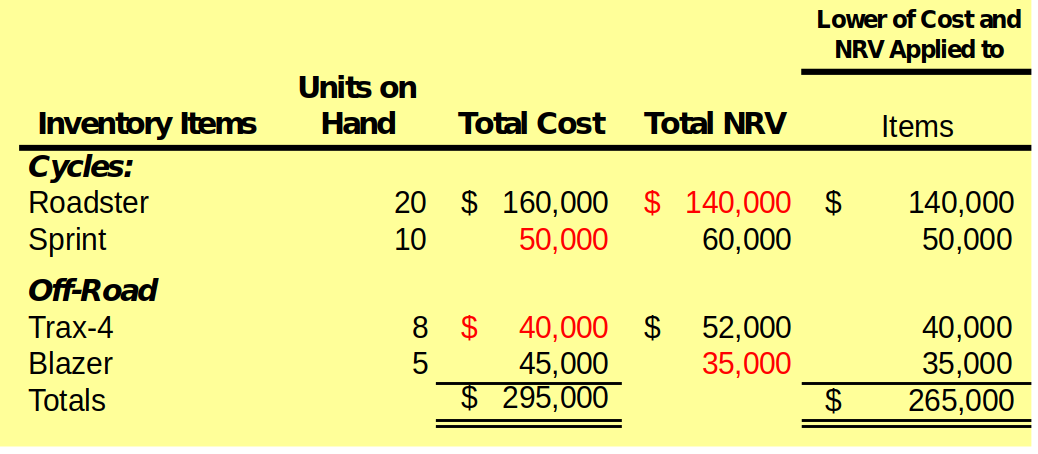
\includegraphics[width=\columnwidth]{images/c7/lcm_eg.png}
	\end{figure}
	
	Inventory must be adjusted downward when NRV is less than cost. To 
	illustrate, if lower of cost and NRV is applied to the individual items of 
	inventory in the exhibit, the Merchandise Inventory account must be adjusted
	
	\begin{figure}[ht]
		\centering
		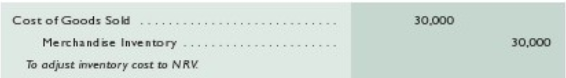
\includegraphics[width=\columnwidth]{images/c7/nrv_adjustment.png}
	\end{figure}
	
	\subsection{Determining Inventory Items}
	
	Merchandise inventory includes all goods that a company owns and holds for 
	sale, regardless of where the goods are located when inventory is counted. 
	We must pay special attention to include inventory that we own but that is 
	in transit or on consignment. We should also consider the condition of 
	inventory that is damaged or obsolete when determining a cost for the 
	inventory.
	
	\subsubsection{Transportation Costs}
	
	Transportation costs are sometimes included in the cost of Merchandise 
	Inventory. The FOB terms designate when title passes and who pays the 
	transportation costs. FOB stands for “\textbf{Free On Board}.”  So, if the 
	shipping terms are Free On Board shipping point, that means that ownership 
	transfers from the seller to the buyer when the seller provides the goods 
	to the carrier.  It also means the buyer will pay all transportation 
	costs.  In this case, the transportation costs will be added to the 
	merchandise inventory account
	
	\subsubsection{Goods on Consignment}
	
	\textbf{Goods on consignment} are goods that are owned by the 
	\textbf{consignor}, but are on 
	display for sale at another place of business \ie the \textbf{consignee}’s. 
	Even 
	though these goods are not in the consignor’s physical possession, the 
	consignor still have ownership of them and should include them in their 
	inventory count.
	
	\subsubsection{Financial Statement Effects of Inventory Errors}
	
	\begin{figure}[ht]
		\centering
		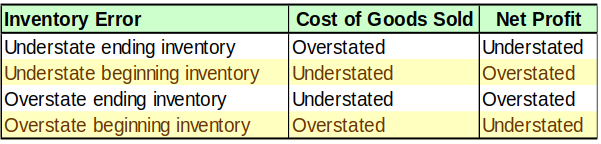
\includegraphics[width=\columnwidth]{images/c7/inventory_error_effects.png}
	\end{figure}
	
\end{document}